\chapter{Implementation}
\label{ch:implementation}

The previous chapters describe FRI and the polynomial commitment scheme
in abstract terms, using oracles and queries. This chapter describes how
they are actually implemented in code. We present the structure of the
implementation, the cryptographic building blocks, the optimisations
added to the basic protocol, and the concrete parameters and the
security level they give.

The implementation is written in Python and uses no external
cryptographic libraries: the field arithmetic, the hash function, the
Merkle commitments, and the Fiat-Shamir challenger are all written from
scratch.


% ==================================================================
\section{Architecture}
\label{sec:impl_architecture}
% ==================================================================

The code is split into modules, each responsible for one part of the
system.

\begin{itemize}
  \item \texttt{field.py} defines the BabyBear prime field: modular
    arithmetic, inversion by Fermat's little theorem, and the two-adic
    generators used to build evaluation domains.
  \item \texttt{extension.py} defines the quartic extension $\Fpk$ over
    the irreducible polynomial $X^4 - 11$, from which the folding
    challenges are drawn.
  \item \texttt{polynomial.py} provides the Number Theoretic Transform,
    the coset low-degree extension, and polynomial evaluation.
  \item \texttt{keccak.py} implements the Keccak-$f$[1600] permutation.
  \item \texttt{merkle\_tree.py} builds Merkle trees over codewords and
    produces and checks authentication paths.
  \item \texttt{challenger.py} implements the duplex-sponge Fiat-Shamir
    transcript on top of the Keccak permutation.
  \item \texttt{fri.py} ties the above together into the commit phase,
    the query phase, and verification.
\end{itemize}

These modules map onto the theory: \texttt{field}, \texttt{extension}
and \texttt{polynomial} realise the algebraic objects of
\cref{ch:background}; \texttt{merkle\_tree} and \texttt{challenger}
realise the BCS transformation of \cref{sec:bcs}; and \texttt{fri}
realises the protocol of \cref{ch:fri}.


% ==================================================================
\section{Cryptographic Components}
\label{sec:impl_crypto}
% ==================================================================

Two roles are served by hashing, and the implementation uses a different
primitive for each, as anticipated in \cref{sec:hash_functions}: SHA-256
for the Merkle commitments, where only collision resistance is needed,
and a Keccak-based duplex sponge for the Fiat-Shamir challenger.

\subsection{Merkle Commitments}
\label{subsec:impl_merkle}

The oracles of the FRI IOP are realised as Merkle vector commitments.
For each layer the prover hashes every codeword entry into a leaf with
SHA-256, builds the binary tree, and publishes the root. A query at a
position is answered with the entry together with its authentication
path, and the verifier recomputes the root as in \cref{fig:merkle}. This
is exactly the ``oracles become commitments, queries become openings''
mechanism of the BCS transformation.

\subsection{The Duplex-Sponge Challenger}
\label{subsec:impl_challenger}

The Fiat-Shamir challenges are produced by a challenger that maintains a
transcript and derives every challenge from it, so that the verifier can
reproduce the same challenges offline. The construction used is a
\emph{duplex sponge}. Chiesa and Orr\`{u}~\cite{CO25} show that a duplex
sponge is a sound basis for Fiat-Shamir, whereas a Merkle-Damg\r{a}rd
hash such as SHA-256 lacks a comparable proof in this setting, which is
why the challenger uses Keccak rather than SHA-256.

The sponge keeps a state that is split into a public \emph{rate}, into
which data is absorbed and from which output is squeezed, and a hidden
\emph{capacity}, which carries the security (\cref{fig:sponge}). Concretely the state is the
$1600$-bit Keccak state, viewed as $25$ lanes of $64$ bits; the first
$17$ lanes ($136$ bytes) are the rate and the remaining $8$ lanes
($64$ bytes) the capacity. Absorbing XORs bytes into the rate and applies
the permutation when the rate fills; squeezing reads bytes back out,
permuting again when the rate is exhausted.

\begin{figure}[ht]
\centering
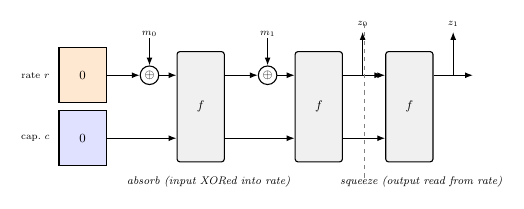
\includegraphics[width=0.92\textwidth]{images/sponge_preview.png}
\caption{The duplex sponge. In the \emph{absorb} phase each input block
$m_i$ is XORed into the rate and the state is passed through the
permutation $f$; in the \emph{squeeze} phase output blocks $z_i$ are read
from the rate, applying $f$ again between reads. The capacity is never
read from or written to directly, which is what carries the security of
the construction.}
\label{fig:sponge}
\end{figure}

The transcript is written and read in a fixed order, which the verifier
must reproduce exactly: the parameters are absorbed first, then for each
round the Merkle root is absorbed and the folding challenge squeezed, and
after the last fold the final layer is absorbed; the query indices are
squeezed once the whole commit transcript is fixed. Two kinds of
challenge are drawn from the squeezed bytes: the folding challenges,
which are elements of $\Fpk$ obtained from sixteen squeezed bytes read as
four base-field coefficients, and the query indices, obtained by reducing
squeezed bytes modulo the domain size. The whole Keccak permutation is
implemented from scratch, so the challenger depends on no external
library.

\FloatBarrier

% ==================================================================
\section{Optimisations}
\label{sec:impl_optimisations}
% ==================================================================

The base protocol of \cref{ch:fri} admits several standard
optimisations. They do not change what the protocol proves; they reduce
proof size or prover work.

\paragraph{Early stopping of the final layer.}
Rather than folding all the way down to a single constant, the prover
stops once the codeword reaches a small fixed length and sends the whole
remaining layer in the clear. This is governed by the parameter
\texttt{final\_poly\_len}: folding continues while the codeword is longer
than \texttt{final\_poly\_len}. The choice trades rounds against the size of
the final layer. For a polynomial of $8$ coefficients with blowup $2$
the initial codeword has $N = 16$ entries, and the options are:
%
\begin{center}
\begin{tabular}{cccc}
\hline
\texttt{final\_poly\_len} & rounds & Merkle roots & final values sent \\
\hline
$1$ & $4$ & $4$ & $1$ \\
$2$ & $3$ & $3$ & $2$ \\
$4$ & $2$ & $2$ & $4$ \\
$8$ & $1$ & $1$ & $8$ \\
\hline
\end{tabular}
\end{center}
%
Each step up the target length removes one round, and with it one Merkle
commitment and its query openings, at the cost of doubling the number of
values sent in the clear at the end. The value $\texttt{final\_poly\_len}
= 2$ used here keeps most of the rounds while sending only two final
values.

\paragraph{Proof-of-work grinding.}
A second, standard optimisation is \emph{grinding}, which buys security
without adding queries~\cite[Section~3.11.3]{ethSTARK}. Before the query
positions are fixed, the prover must find a \emph{nonce} whose hash begins
with $g$ zero bits, costing about $2^{g}$ hash attempts. An honest prover
does this once; a cheating prover, whose attack is a retry loop that needs
a fresh transcript, and hence a fresh nonce, at every attempt, pays it
each time. This multiplies the attacker's effort by $2^{g}$, adding $g$
bits on top of the query term:
%
\begin{equation}
\label{eq:security_with_grinding}
\lambda \;=\; \underbrace{s \cdot \tfrac{1}{2}\log_2(1/\rho)}_{\text{from the queries}}
\;+\; \underbrace{g}_{\text{from grinding}} .
\end{equation}
%
This optimisation is present in our implementation only as a stub, with an
empty proof-of-work routine and the difficulty fixed to zero, so it adds
nothing here ($g = 0$).


% ==================================================================
\section{Parameters and Security Level}
\label{sec:impl_parameters}
% ==================================================================

The soundness bound of \cref{thm:rbr} turns the choice of parameters into
a choice of security level. Its two error terms are the folding term
$\tfrac{r}{|\mathbb{K}|}\cdot\mathrm{poly}(|D|)$, which depends on the
size of the challenge field, and the query term $(1-\delta)^{s}$, which
depends on the number of queries $s$ and the distance $\delta$. Because
challenges are drawn from the quartic extension $\Fpk$, with
$|\mathbb{K}| = p^4 \approx 2^{124}$, the folding term is at most about
$2^{-122}$ for the round counts used here and is never the bottleneck.
The security level is therefore set by the query term.

In the provable regime the distance is bounded by the Johnson radius
$\delta < 1 - \sqrt{\rho}$ (\cref{thm:johnson}), and each query
contributes
%
\begin{equation}
\label{eq:bits_per_query}
-\log_2(1-\delta) \;=\; \tfrac{1}{2}\log_2(1/\rho)
\end{equation}
%
bits of security, so $s$ queries give $\tfrac{s}{2}\log_2(1/\rho)$ bits.
The rate $\rho$ thus controls how much each query is worth: a smaller
rate (a larger blowup factor) buys more bits per query, at the cost of a
larger evaluation domain and more prover work.

Since grinding is not enabled in our configuration
(\cref{sec:impl_optimisations}), the security level here comes entirely
from the queries; the early-stopping optimisation does not affect it, as
it only trades rounds against the length of the final layer and so changes
the proof size rather than the security level.

\paragraph{Parameters used in this work.}
The configuration evaluated here is
%
\[
\texttt{log\_blowup} = 1,\quad
\texttt{num\_queries} = 20,\quad
\texttt{proof\_of\_work\_bits} = 0,\quad
\texttt{final\_poly\_len} = 2 .
\]
%
Here \texttt{final\_poly\_len} sets the early-stopping point and
\texttt{proof\_of\_work\_bits} the grinding difficulty of
\cref{sec:impl_optimisations}. The rate is $\rho = 1/2$, so by
\cref{eq:bits_per_query} each query is worth $0.5$ bits and the $20$
queries provide about $10$ bits; grinding is set to $0$, so by
\cref{eq:security_with_grinding} it adds nothing and the security comes entirely
from the queries. This is deliberately a \emph{test} configuration, chosen so that proofs are small and fast to generate while
exercising every part of the protocol; it is not a production security
level.

\paragraph{Reaching a production level.}
The security level is raised by lowering the rate, which increases the
bits per query: at $\rho = 1/8$ each query is worth $1.5$ bits, and at
$\rho = 1/16$ it is worth $2$ bits. A typical production target of
$100$ bits is reached, for example, with a blowup of $16$ and around
$50$ queries. In general, the number of queries needed to reach a target
of $\lambda$ bits is obtained by inverting
\cref{eq:bits_per_query}:
%
\begin{equation}
\label{eq:queries_for_target}
s \;=\; \frac{\lambda}{\tfrac{1}{2}\log_2(1/\rho)} .
\end{equation}
%
For $\lambda = 100$ this gives $100/0.5 = 200$ queries at $\rho = 1/2$,
$100/1.5 \approx 67$ at $\rho = 1/8$, and $100/2 = 50$ at $\rho = 1/16$.
The following table summarises the trade-off.

\begin{center}
\begin{tabular}{lcccc}
\hline
 & blowup & $\rho$ & bits/query & queries for $100$ bits \\
\hline
This work (test) & $2$  & $1/2$  & $0.5$ & $\approx 200$ \\
Moderate         & $8$  & $1/8$  & $1.5$ & $\approx 67$ \\
Aggressive       & $16$ & $1/16$ & $2.0$ & $\approx 50$ \\
\hline
\end{tabular}
\end{center}

The query counts in the last column assume no grinding; enabling
grinding of $g$ bits would lower each of them by $g$ divided by the bits
per query. The table makes the central trade-off explicit: a larger
blowup makes each query more powerful, so fewer are needed, but it
enlarges the committed codeword and so raises the prover's cost and the
proof size. The test parameters sit
at the cheap, low-security end of this spectrum, which is appropriate for
validating correctness but would be raised for any real deployment.


% ==================================================================
\section{The Polynomial Commitment Scheme}
\label{sec:impl_pcs}
% ==================================================================

The polynomial commitment scheme of \cref{ch:pcs} is implemented in
\texttt{pcs.py} as a thin layer over the FRI prover and verifier. It
exposes the three operations \texttt{commit}, \texttt{open\_at} and
\texttt{verify}, and reuses the FRI machinery for the low-degree test on
the quotient.

\texttt{commit} evaluates $f$ on the low-degree extension coset, hashes
each entry into a Merkle leaf with SHA-256, and returns the root together
with the prover's copy of the codeword and tree.

\texttt{open\_at} implements the quotient technique. It first rejects any
evaluation point $z$ that lies in the coset domain: since the domain is a
coset $g\langle\omega\rangle$ with $g^N = -1$, the check is $z^N \neq
g^N$, and if it fails the quotient would require dividing by zero at a
domain point. It then forms the quotient coefficients of
\cref{eq:quotient} by the synthetic division
%
\[
q_{d-1} = a_d, \qquad q_{i-1} = a_i + z\,q_i \quad (i = d-1, \ldots, 1),
\]
%
where $a = f - v$, runs the FRI prover on $q$, and opens the committed
$f$ at the same query positions FRI used on $q$. Those positions are
recovered by replaying the Fiat-Shamir transcript exactly as the verifier
will, so both sides agree on the same indices without further
communication.

\texttt{verify} runs the FRI verifier on the quotient proof, then at each
queried position $x$ checks the consistency relation in the form used by
the code,
%
\begin{equation}
\label{eq:pcs_check}
q(x)\,(x - z) = f(x) - v,
\end{equation}
%
which is the check of \cref{eq:quotient_check}, using the opened value of
$f$ checked against the commitment root and the value of $q$ taken from
the first FRI layer. Acceptance requires the FRI proof to verify and
\cref{eq:pcs_check} to hold at every queried position.

The scheme is exercised by a small test suite in \texttt{test\_pcs.py}:
an honest opening of $f$ at a point outside the domain is accepted, a
claim with a wrong value is rejected, and an opening with a tampered $f$
value is rejected.

% ==================================================================
\section{Testing}
\label{sec:impl_testing}
% ==================================================================

Correctness is checked by a small test suite. An honest prover is run
end to end and its proof is accepted. Two dishonest provers are then
constructed, one that corrupts a committed value and one that corrupts
the final layer, and in both cases verification rejects, confirming that
the colinearity checks catch inconsistencies. The Number Theoretic
Transform is checked independently against direct evaluation of the same
polynomial, ensuring the coefficient-to-evaluation conversion is correct.